\documentclass[12pt, letterpaper]{report}
\usepackage[UTF8]{ctex}
\usepackage{plantuml}
\usepackage{tikz}
\usepackage{amsmath}
\usepackage{tikz-uml}
\usepackage{comment}
\usepackage{amssymb}
\usepackage{algorithm}
\usepackage{algpseudocode}
\usepackage{hyperref}
\usepackage{booktabs}
\usepackage{multirow}
\usetikzlibrary{positioning}
\usetikzlibrary{shapes.multipart}
\usepackage{svg}
\usepackage[pdf]{graphviz}
\usepackage{listings}
\usepackage{fancyvrb}
\lstset
{ %Formatting for code in appendix
    language=C++,
    basicstyle=\ttfamily,
    numbers=left,
    stepnumber=1,
    showstringspaces=false,
    tabsize=1,
    breaklines=true,
    breakatwhitespace=false,
    escapechar=|
}

%\usepackage{algorithmic}
\begin{document}
\title{机密计算抽象}
\author{高炜贺}
\date{2023-12-29}
\maketitle

\newpage

\chapter{可信计算环境的功能和特性}

本文分析基于可信计算环境(TEE)的机密计算(CC),找出众多TEE原型的异同,最终尝试抽象出其共有API集合。面向CC的TEE,通常至少有以下几个特性或功能。

\begin{enumerate}
    \item 内存隔离\\
    内存隔离通过安全硬件,保证数据和指令不被篡改。大多数情况下,我们在思考时,假定TEE在硬件层面是安全的。因此,侧信道攻击(SCA)不在本文讨论范围内。但是,SCA其实是最广泛应用的TEE攻击手段,也是TEE最薄弱的环节。

    \begin{lstlisting}
// untrusted memory ops 
bytes u_mem_rd(src_addr, length); 
u_mem_wr(dest_addr, bytes, length); 
        
// trusted memory ops
bytes t_mem_rd(src_addr, length);
t_mem_wr(dest_addr, bytes, length);         
    \end{lstlisting}

    \item 可信认证\\
    可信认证(attestation)通过可信硬件,以及一套安全的认证协议,证明TEE内的数据和代码未被篡改。这一功能可分为本地可信认证(LA)和远程可信认证(RA)。不同应用场景,对二者的需求不同。例如,类似YPC的OLAP框架通常至少需要依赖RA;但早期PC上的蓝光4K播放并不依赖实时的在线RA。

    \begin{lstlisting}
// attestations 
Report local_attest(
    TargetInfo target_info
) {
    // 1. generate report within target enclave
    // 2. send the report to attesting enclave
    // 3. retrieve report from attesting enclave and return 
}; 
Report remote_attest(
    TargetInfo target_info
) {
    // 1. generate report in target enclave
    // 2. send report to QE
    // 3. retrieve RA report and return
};   
    \end{lstlisting}

    \item 可信密钥\\
    TEE与可信平台模块(TPM)类似,也需要具备至少一个信任根EK。EK通常为设备相关的密钥。TEE设备行为的可信性认证,由该密钥签发。EK还可以生成更多的子密钥,以支持更加灵活的功能。显而易见地,这些子密钥依赖于平台信任根EK。

    \begin{lstlisting}
// Endorsement key 
Certificate get_ek_certificate(); 
    \end{lstlisting}

    \item 可信输入输出\\
    为了提高外设(也包括部分总线设备)在TEE场景下的性能,一些(尤其是面向虚拟机的)TEE设计方案在逻辑上支持与裸金属(bare-metal)虚拟机类似的硬件直通。该功能一般称为可信输入输出(Trusted I/O)。它通常是通过计算机总线加密,或通信线缆加密实现。
\end{enumerate}

一些TEE的实现可能只具备上述功能的一部分,也有一些产品支持更多扩展功能。这些差异,都不影响其被认为是TEE。但是,面向OLAP功能的TEE,一般至少要支持类似的功能,以提供特定场景下的安全性和可用性。本文以上述四个功能为基础,首先抽象其对应的API,然后尝试将其组合起来,构成与YPC类似的功能实现。
\chapter{YPC的功能模块}

YPC在可信域和不可信域均有重要的功能和协议设计。本章试图模块化地抽象YPC,找出各组件之间的联系和依赖关系。从这些依赖关系中,找出与TEE各功能的对应关系,进而得出YPC对于TEE的依赖情况。

\begin{figure}
    \centering
    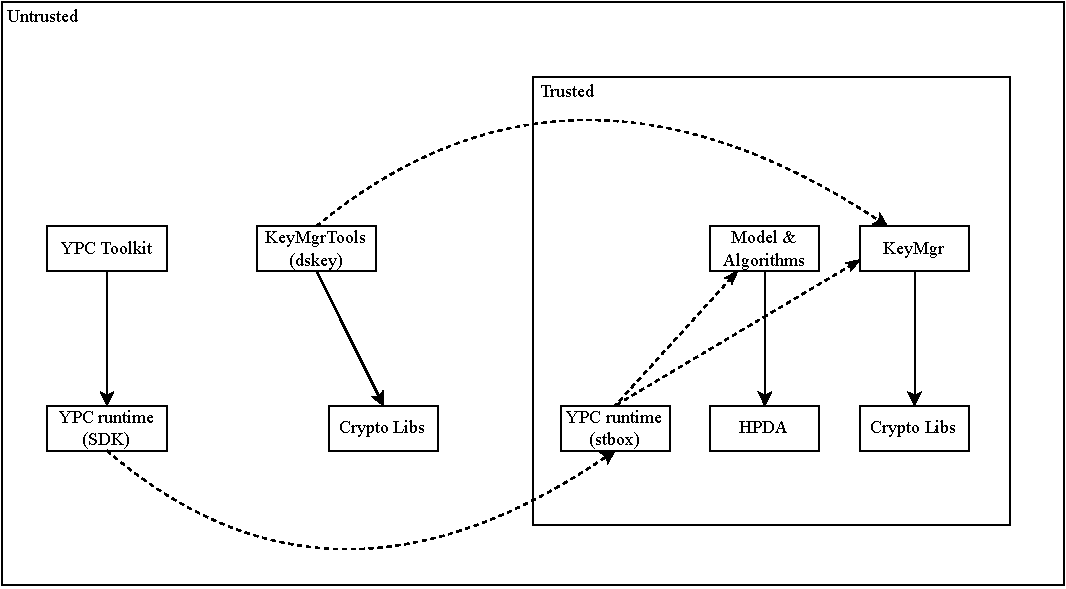
\includegraphics[width=140mm]{figure/ypc-modular.pdf}
    \caption{YPC模块关系图。整个系统分为两个区域,二者信任模型不同:其中Trusted为可信域,在TEE中存储和执行;Untrusted为不可信域,在TEE外执行。两个区域各有运行时(runtime)用于同步数据和系统状态。}
    \label{fig:ypc-modular}
\end{figure}

图\ref{fig:ypc-modular}展示了YPC的模块化框图。在初始化阶段,运行在非可信域中的KeyMgrTools将由EK加密后的平台相关密钥信息,通过可信信道传输到可信域中的KeyMgr中。

$S^D_c = seal_{EK}(S^D_p)$

$S^D_p = unseal_{EK}(S^D_c)$

从协议角度,YPC的简化模型包括四个角色,
\begin{enumerate}
    \item 数据提供方(data provider)\\ 
    提供任务图中的原始数据,以自己持有的枢公钥加密原始数据。
    \item (算法)模型提供方(model provider)\\ 
    开发者,算法提供方也可以提供相应的模型。
    \item 数据使用方(data user)\\ 
    得到最终的计算任务输出。
    \item 算力提供方,又称计算平台(computing platform)\\ 
    安装Fidelius隐私计算节点,持有典公钥。
\end{enumerate}

YPC支持的机密计算功能和特性包括,本地数据可用不可见、托管数据可用不可见、结果的可信性证明、结果不可见、数据用途限制、模型不可见、模型用途限制、任务参数不可见、原子交付。

本文描述YPC部分特性的实现方法,并以伪代码形式展示。

\begin{enumerate}
    \item 本地数据可用不可见\\
    本地数据可通过加密后存储到外设上。

    \begin{lstlisting}
bytes local_data; 
bytes encrypted_data = encrypt(local_data, 
    platform_pkey);
t_mem_wr(epc_addr, 
    local_data, local_data.length); 
    \end{lstlisting}

    \item 托管数据可用不可见\\
    将数据加密后,托管到第三方存储。

    \begin{lstlisting}
bytes local_data; 
bytes encrypted_data = encrypt(local_data, dest_pkey); 
// upload to delegatee storages
        
// download from delegatee storages
bytes delegated_data; 
bytes dest_pk; 
t_mem_wr(dpk_epc_addr, 
    dest_pk, dest_pk.length); 
t_mem_wr(dd_epc_addr, 
    delegated_data, delegated_data.length);   
    \end{lstlisting}

    \item 结果的可信性证明\\ 
    计算平台得到计算结果后,通过$S^D$对结果签名,保证计算结果的正确性完整性。

    \begin{lstlisting}
// Executed in TEE
Report report; 
report = local_attest(model_einfo); 
// send report to keymgr enclave
    \end{lstlisting}

    \item 结果不可见\\ 
    计算平台得到计算结果后,将结果加密后,返回数据使用方。

    \begin{lstlisting}
// Executed in TEE
bytes result; 
bytes encrypted_result = encrypt(result, du_pkey); 
    \end{lstlisting}

    \item 数据用途限制\\ 
    (还未实现)计算平台解析元数据,检查数据用途。
    \begin{lstlisting}
// Check params in model enclave
    \end{lstlisting}
    \item 模型不可见\\ 
    模型源代码不可见,仅将编译后的二进制文件传入计算平台。

    \begin{lstlisting}
// Signed dynamic library

// Possible implementations in the future: 
bytes model_so; 
bytes encrypted_model = encrypt(model_so, platform_pkey); 
    \end{lstlisting}

    \item 模型用途限制\\ 
    计算平台解析模型元数据,检查模型参数和用途。

    \begin{lstlisting}
// Check params in model enclave
    \end{lstlisting}

    \item 任务参数不可见\\ 
    数据使用方将计算任务参数加密后,传入计算平台。
    
    \begin{lstlisting}
// Encrypt params with platform pkey
    \end{lstlisting}
    
    \item 原子交付\\
    通过智能合约,保证任务结果交付和任务费用交付的原子性绑定。

    \begin{lstlisting}
// Chains and smart contracts
    \end{lstlisting}

\end{enumerate}


\chapter{结论}

本文希望将YPC普适性地扩展到众多TEE实现的框架。


\end{document}